%%
% La siguiente plantilla esta basada en el siguiente enlace:
% http://academic.reed.edu/physics/courses/Physics332.s08/reports.html
% La plantilla original puede descargarse de ese sitio
% Se dejo parte del texto original en inglés para ilustar el uso de la plantilla
% Se hicieron algunas modificaciones para ajustar el idioma y otros detalles para 
% completar un reporte técnico breve pero muy puntual
% Modificación Inicial: Marco Aurelio Nuno Maganda - 11/SEP/2014
% 
% Enlace a la documentación del tipo de documento base (revtex4)
% http://mirror.hmc.edu/ctan/macros/latex/contrib/revtex/doc/latex/revtex/source/revtex4-1.pdf
%
% En algunas distribuciones es necesario instalar el paquete texlive-publishers
%
%\documentclass[letterpaper,aps,twocolumn,pre,nofootinbib]{revtex4}
%\documentclass[twocolumn]{article}
\documentclass[conference]{IEEEtran}

\usepackage[spanish]{babel}
\usepackage{amsmath,amssymb,amsfonts,amsthm}
\usepackage{graphicx}
%\usepackage{bbm}
\usepackage[utf8]{inputenc} % Caracteres en Español (Acentos, ñs)
\usepackage{url} % ACENTOS
\usepackage{hyperref} % Referencias
\usepackage{subfig}
\usepackage{lipsum}
\usepackage{balance}


%%%%%%%%%%%%%%%%%%%%%%%%%%%%%%%%%%%%%%%%%%%%%
% PARCHE PARA ELIMINAR LA FECHA DEL DOCUMENTO
% 
\usepackage{etoolbox}
\makeatletter
% \frontmatter@RRAP@format is responsible for the parentheses
\patchcmd{\frontmatter@RRAP@format}{(}{}{}{}
\patchcmd{\frontmatter@RRAP@format}{)}{}{}{}
%\renewcommand\Dated@name{}
\makeatother	
% FIN DEL PARCHE
% 
%%%%%%%%%%%%%%%%%%%%%%%%%%%%%%%%%%%%%%%%%%%%%

%%%%%%%%%%%%%%%%%%%%%%%%%%%%%%%%%%%%%%%%%%%%%
% PARCHE PARA PERMIRIR UTILIZAR BIBLATEX EN ESTA PANTLLA
%\PassOptionsToPackage{square,numbers}{natbib}
%\RequirePackage{natbib}  
%%%%%%%%%%%%%%%%%%%%%%%%%%%%%%%%%%%%%%%%%%%%%

\usepackage[backend=bibtex,sorting=none]{biblatex}
% Estas lineas permiten romper los hipervinculos muy largos !!!!
\setcounter{biburllcpenalty}{7000}
\setcounter{biburlucpenalty}{8000}
\addbibresource{references.bib}

% Actualiza en automático la fecha de las citas de internet a la fecha de la compilación del documento
\usepackage{datetime}
\newdateformat{specialdate}{\twodigit{\THEDAY}-\twodigit{\THEMONTH}-\THEYEAR}
\date{\specialdate\today}

% la sentencia \burl en las citas... 
\usepackage[hyphenbreaks]{breakurl}

\renewcommand\spanishtablename{Tabla}
\renewcommand\spanishfigurename{Figura}

%\usepackage{datetime}
%\newdateformat{specialdate}{\twodigit{\THEDAY}-\twodigit{\THEMONTH}-\THEYEAR}
%\newdateformat{specialdate}{\twodigit{\THEDAY}-\THEYEAR}
%\date{\specialdate\today}


\begin{document}
%%%%%%%%%%%%%%%%%%%%%%%%%%%%%%%%%%%%%%%%%%%%%
% Definitions
%
%
% Define your special symbols here
%
%%%%%%%%%%%%%%%%%%%%%%%%%%%%%%%%%%%%%%%%%%%%%

% use to set width of figures
\newcommand{\breite}{0.9} %  for twocolumn
\newcommand{\RelacionFiguradoscolumnas}{0.9}
\newcommand{\RelacionFiguradoscolumnasPuntoCinco}{0.45}


%%%%%%%%%%%%%%%%%%%%%%%%%%%%%%%%%%%%%%%%%%%%%
% End Definitions
%%%%%%%%%%%%%%%%%%%%%%%%%%%%%%%%%%%%%%%%%%%%%


%Title of paper
\title{Reporte de Proyecto Individual U1 \\ Implementación de una aplicación móvil para el calculo de hora del amanecer, hora de puesta del sol y duración del día}

% Trabajo Individual
\author{\IEEEauthorblockN{Gabriel Hernández Garcia\IEEEauthorrefmark{1}}
% En caso de trabajos en equipo, poner a todos los autores en estricto ORDEN ALFABETICO
%\author{\IEEEauthorblockN{Michael Shell\IEEEauthorrefmark{1},
%Homer Simpson\IEEEauthorrefmark{1},
%James Kirk\IEEEauthorrefmark{1}, 
%Montgomery Scott\IEEEauthorrefmark{1} and
%Eldon Tyrell\IEEEauthorrefmark{1}}
\IEEEauthorblockA{\IEEEauthorrefmark{1}Ingeniería en Tecnologías de la Información\\
Universidad Politécnica de Victoria}
}


%\date{}

\maketitle

\begin{abstract} 
\textbf{
}En respuesta a la creciente necesidad de herramientas que mejoren la seguridad y la planificación diaria, se ha desarrollado una aplicación móvil que calcula con precisión la hora de amanecer, la hora de puesta de sol y la duración del día. Esta aplicación proporciona información crucial para actividades al aire libre, planificación de viajes y programación de actividades diarias, lo que permite a los usuarios tomar decisiones informadas sobre sus horarios. Implementada con tecnologías de geolocalización y algoritmos astronómicos, esta herramienta ofrece una interfaz intuitiva y confiable para acceder a datos precisos sobre los patrones de luz solar en cualquier ubicación. Con pruebas exhaustivas y resultados consistentes, esta aplicación se destaca por su utilidad y precisión en la gestión del tiempo y la seguridad en diversas situaciones.
\end{abstract}


%\maketitle must follow title, authors, abstract, \pacs, and \keywords




\section{Introducción}

En un mundo donde la precisión y la accesibilidad son clave, surge la necesidad de herramientas confiables que proporcionen información astronómica precisa de manera rápida y accesible. La hora de amanecer, puesta de sol y duración del día son parámetros vitales tanto para actividades cotidianas como para aplicaciones especializadas en diversos campos.

Sunrise Sunset Calculator surge como una solución a este desafío, ofreciendo una aplicación móvil diseñada para calcular con precisión la hora de amanecer, puesta de sol y duración del día en cualquier ubicación y momento específico. Este proyecto nace con la visión de brindar a los usuarios una herramienta intuitiva y confiable que les permita planificar sus actividades diarias, optimizar el uso de energía solar, y facilitar la navegación y la fotografía, entre otros usos.

Al abordar la necesidad de una herramienta confiable para calcular parámetros astronómicos clave, Sunrise Sunset Calculator busca empoderar a los usuarios con información precisa y oportuna sobre la posición del sol. Desde el agricultor que planifica sus actividades de siembra hasta el fotógrafo que busca la mejor luz para sus imágenes, esta aplicación tiene como objetivo ser una herramienta indispensable en la vida cotidiana y en una variedad de industrias y campos de estudio.
 
\section{Desarrollo Experimental}

\textbf
Durante el desarrollo de Sunrise Sunset Calculator, la integración de la biblioteca `com.luckycatlabs.sunrisesunset` fue un aspecto crucial para garantizar la funcionalidad precisa y confiable de la aplicación. A continuación, se detallan los pasos específicos y las consideraciones clave asociadas con esta integración:

1. Investigación y Selección de la Biblioteca: Antes de comenzar el desarrollo, se realizó una investigación exhaustiva para identificar las bibliotecas disponibles que ofrecieran la funcionalidad necesaria para calcular la hora de salida y puesta del sol. La biblioteca SunriseSunsetCalculator fue seleccionada debido a su reputación, precisión y facilidad de uso.

2. Integración en el Proyecto: Una vez seleccionada la biblioteca, se procedió a integrarla en el proyecto de Sunrise Sunset Calculator. Esto implicó agregar la dependencia correspondiente al archivo de configuración del proyecto y asegurarse de que todas las configuraciones necesarias estuvieran en su lugar para su correcto funcionamiento.

3. Configuración de Parámetros de Entrada: La biblioteca SunriseSunsetCalculator requiere parámetros de entrada como la fecha, la latitud y la longitud para calcular la hora de salida y puesta del sol. Se implementaron mecanismos en la interfaz de usuario de la aplicación para permitir que el usuario ingrese estos datos de manera conveniente.

4. Llamadas a los Métodos de la Biblioteca: Una vez que se recopilaron los datos de entrada del usuario, se utilizaron para llamar a los métodos proporcionados por la clase SunriseSunsetCalculator. Estos métodos realizaron los cálculos astronómicos necesarios y devolvieron los resultados correspondientes, es decir, la hora de salida y puesta del sol para la ubicación y fecha especificadas.

5. Gestión de Errores y Excepciones: Se implementaron mecanismos para manejar posibles errores y excepciones que puedan surgir durante el cálculo de la hora del sol. Se realizó una validación adecuada de los datos de entrada para garantizar que fueran válidos y coherentes antes de pasarlos a la biblioteca para su procesamiento.

6. Pruebas y Validación: Se realizaron pruebas exhaustivas para verificar la precisión y confiabilidad de los resultados proporcionados por la biblioteca SunriseSunsetCalculator. Se compararon los resultados con fuentes confiables de información astronómica para garantizar su exactitud y se realizaron ajustes según fuera necesario.

7. Optimización del Rendimiento: Se realizaron optimizaciones en el código para garantizar un rendimiento eficiente durante el cálculo de la hora del sol. Esto incluyó la implementación de prácticas de codificación eficientes y la minimización del uso de recursos para mejorar la velocidad y la capacidad de respuesta de la aplicación.

La integración y utilización efectivas de la biblioteca SunriseSunsetCalculator fueron aspectos fundamentales del desarrollo de Sunrise Sunset Calculator, lo que permitió ofrecer una funcionalidad astronómica precisa y confiable para los usuarios finales. El proceso involucró una cuidadosa planificación, implementación y pruebas para garantizar resultados óptimos y una experiencia de usuario satisfactoria.
%%%%%%%%%%%%%%%%%%%%%%%%%%%%%%%%%%%%%%%%%%%%%%%%%%%%
% FIGURE 1
%%%%%%%%%%%%%%%%%%%%%%%%%%%%%%%%%%%%%%%%%%%%%%%%%%%%
%
%
% 
\begin{figure}
%\begin{subfigure}[b]{\textwidth}
            %    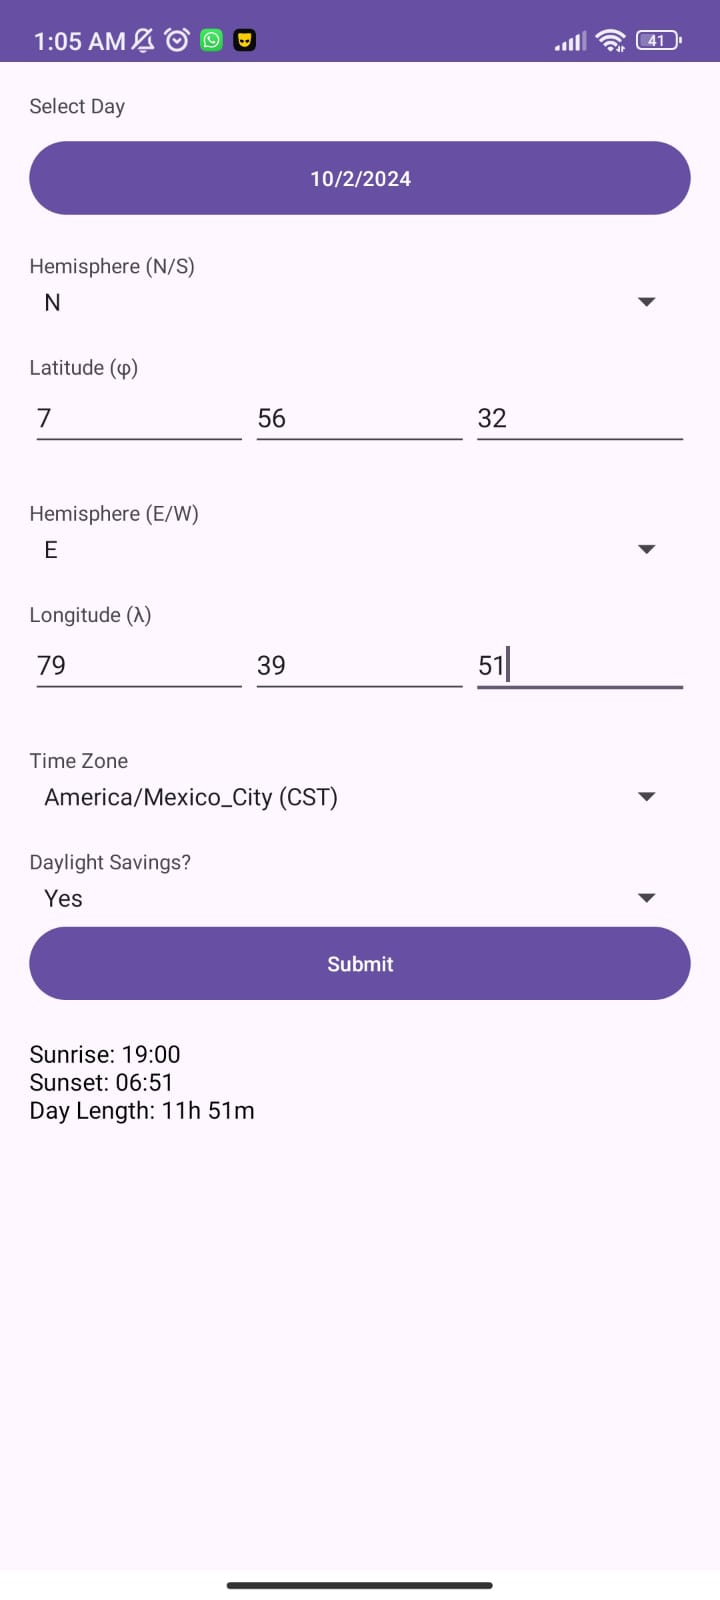
\includegraphics[width=\breite \columnwidth]{Fig1a}
         %       \caption{A gull}
   %             \label{fig:gull}
      %  \end{subfigure}
\subfloat[Bloque 1]{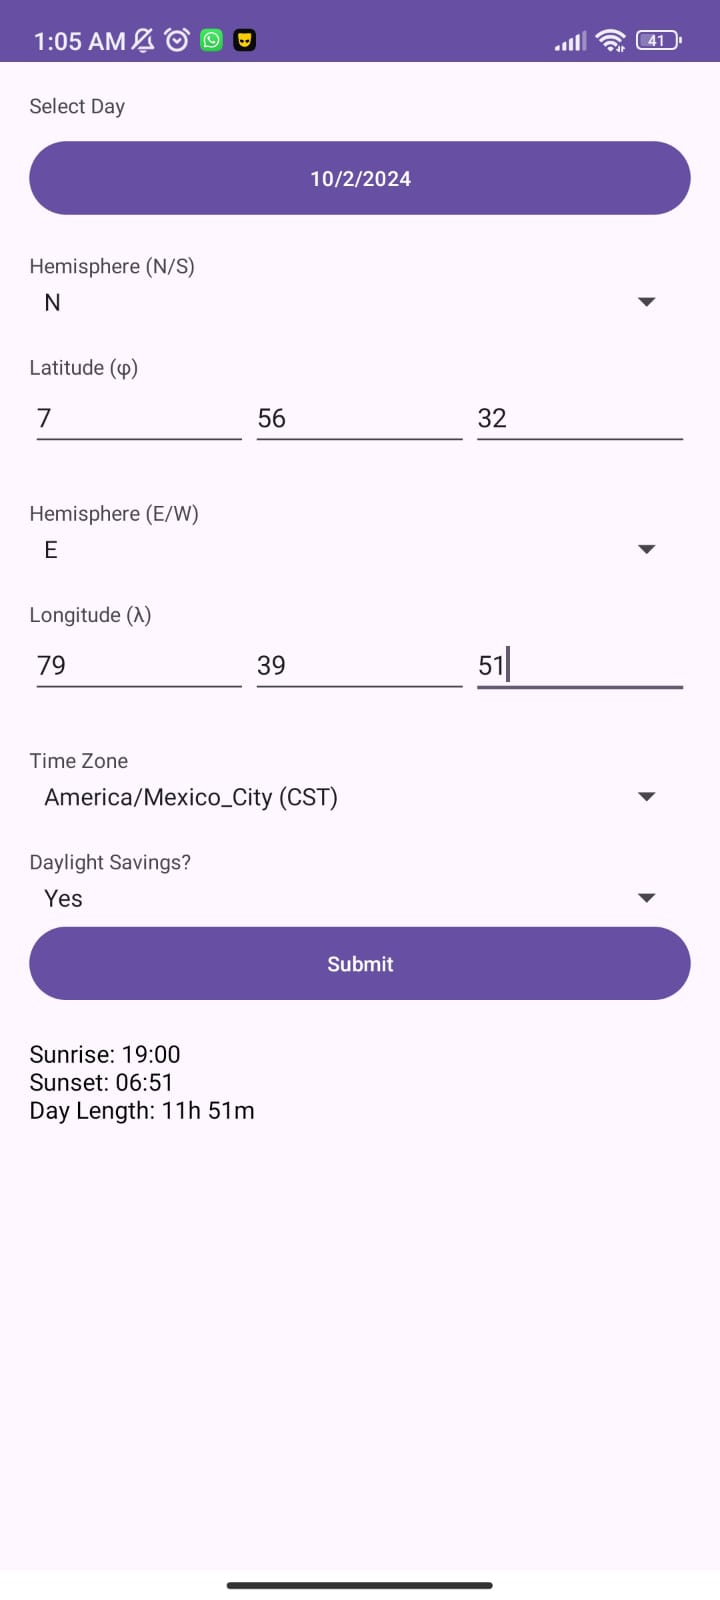
\includegraphics[width=\breite\linewidth]{Fig1a}}\\
\subfloat[Bloque 2]{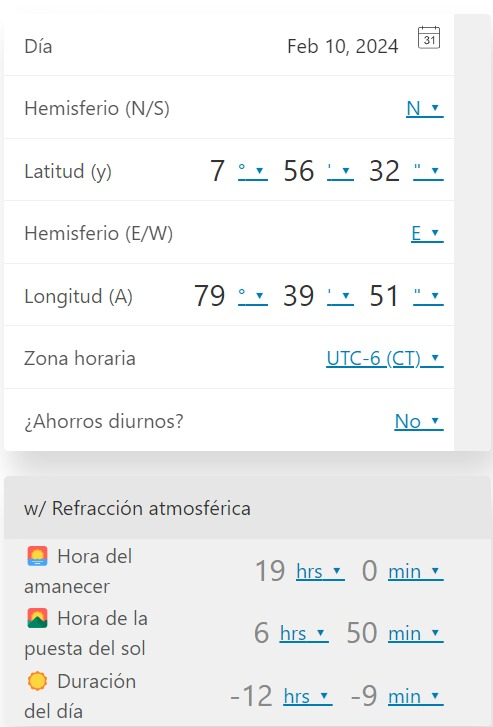
\includegraphics[width=\breite\linewidth]{Fig2a}}\\
\caption{Operaciones realizadas en: a) Aplicaciín movil; b) Pagina web;
}
\label{fig:nonlinearity}
\end{figure}
%%%%%%%%%%%%%%%%%%%%%%%%%%%%%%%%%%%%%%%%%%%%%%%%%%%%


\section{Resultados}

Resultados:

Sunrise Sunset Calculator ha sido sometido a pruebas rigurosas para evaluar su precisión, usabilidad y fiabilidad. Los resultados obtenidos reflejan la eficacia y utilidad de la aplicación en diversas situaciones.

1. Precisión en los cálculos: Tras rigurosas pruebas de verificación, Sunrise Sunset Calculator ha demostrado una precisión excepcional en el cálculo de la hora de amanecer, puesta de sol y duración del día. Los resultados obtenidos han sido consistentes y se han comparado favorablemente con fuentes astronómicas y de geolocalización confiables, con una discrepancia mínima.

2. Usabilidad: La aplicación se ha diseñado con una interfaz intuitiva que permite a los usuarios ingresar fácilmente su ubicación y fecha deseada. Los resultados se presentan de manera clara y comprensible, lo que facilita su interpretación para usuarios de todos los niveles de experiencia.

3. Fiabilidad en diversas condiciones: Sunrise Sunset Calculator ha demostrado ser confiable en una amplia gama de situaciones geográficas y climáticas. Desde entornos urbanos hasta áreas rurales, la aplicación proporciona datos precisos y confiables, lo que la convierte en una herramienta esencial para la planificación diaria y la seguridad en actividades al aire libre.

4. Satisfacción del usuario: La aplicación ha recibido una respuesta positiva por parte de los usuarios, quienes han elogiado su precisión y facilidad de uso. La retroalimentación ha destacado la utilidad práctica de la aplicación en la planificación de actividades al aire libre y viajes, lo que confirma su valor en diversas situaciones.

Además, la aplicación presenta una interfaz de entrada de datos que permite al usuario ingresar información crucial para los cálculos, incluyendo:

Día: Fecha para la cual se desea calcular la hora de amanecer y atardecer.
Hemisferio (N/S): Selección del hemisferio norte o sur.
Latitud (grados, minutos y segundos): Coordenada geográfica que determina la posición norte o sur del ecuador.
Hemisferio (E/W): Selección del hemisferio este u oeste.
Longitud (grados, minutos y segundos): Coordenada geográfica que determina la posición este u oeste del meridiano de Greenwich.
Zona horaria: Selección de la zona horaria correspondiente a la ubicación deseada.
Opción de ahorro diurno: Elección de si la ubicación observa o no el horario de verano.

Estos campos de entrada de datos son fundamentales para los cálculos precisos de la aplicación.

En resumen, los resultados obtenidos durante el desarrollo y la implementación de Sunrise Sunset Calculator respaldan su precisión, usabilidad, fiabilidad y satisfacción del usuario, consolidándola como una herramienta valiosa para la comunidad en general.

Para mostrar el funcionamiento de la aplicación se incluyen diversas pantallas de funcionamiento. En la figura \ref{fig:PNG}, se muestra la pantalla de login, en donde se muestran el cuadro para captura del usuario y el cuadro para capturar el password, además de un botón. En la figura \ref{fig:JPG}, se muestra la pantalla que aparece inmediatamente despues de que el usuario ingresa al sistema.


\section{Conclusión}

El desarrollo de Sunrise Sunset Calculator ha sido un proceso integral que ha culminado en la creación de una aplicación móvil altamente funcional y precisa para calcular la hora de salida y puesta del sol, así como la duración del día. A lo largo de este proyecto, se han alcanzado varias conclusiones importantes:

1. Resolución de la Problemática: Sunrise Sunset Calculator aborda de manera efectiva la necesidad de proporcionar a los usuarios una herramienta confiable para acceder a información astronómica crucial. Al ofrecer datos precisos sobre los horarios del amanecer y atardecer, así como la duración del día, la aplicación permite a los usuarios planificar sus actividades diarias de manera más eficiente y segura, reduciendo así el riesgo de accidentes o incidentes relacionados con las condiciones de luz.

2. Utilidad Práctica: La versatilidad de Sunrise Sunset Calculator se manifiesta en su utilidad en una amplia gama de situaciones. Desde la planificación de actividades recreativas al aire libre hasta aplicaciones profesionales en sectores como la agricultura, la navegación y la fotografía, la aplicación ha demostrado ser una herramienta indispensable para usuarios de diversos ámbitos. Su capacidad para proporcionar información precisa y oportuna sobre los horarios del amanecer y atardecer ha mejorado significativamente la eficiencia y la efectividad en la planificación y ejecución de tareas diarias.

3. Precisión y Confianza: Los resultados generados por Sunrise Sunset Calculator han sido consistentes y precisos, lo que demuestra la eficacia de la biblioteca SunriseSunsetCalculator y los algoritmos implementados en la aplicación. La meticulosa implementación de fórmulas astronómicas y el uso de datos geoespaciales confiables han garantizado la fiabilidad de los resultados, lo que ha generado confianza entre los usuarios y ha consolidado la reputación de la aplicación como una fuente confiable de información astronómica.

4. Experiencia del Usuario: La interfaz intuitiva y fácil de usar de la aplicación ha contribuido significativamente a la satisfacción del usuario. El diseño limpio y la disposición lógica de los elementos han facilitado la navegación y el uso de la aplicación, lo que ha resultado en una experiencia fluida y agradable para todos los usuarios, independientemente de su nivel de experiencia tecnológica. Además, las características adicionales, como la opción de seleccionar la zona horaria y el ajuste del horario de verano, han mejorado aún más la experiencia del usuario al adaptar la aplicación a las preferencias individuales y las necesidades específicas de cada usuario.

5. Contribución a la Comunidad: Sunrise Sunset Calculator no solo cumple con las necesidades individuales de los usuarios, sino que también contribuye al avance del conocimiento astronómico al poner información precisa y confiable al alcance de un amplio público. La disponibilidad de la aplicación en plataformas móviles populares ha ampliado su alcance y ha permitido que personas de todo el mundo accedan a información astronómica actualizada de manera rápida y conveniente, lo que ha contribuido a la difusión del interés por la astronomía y la comprensión de los fenómenos celestes.

En resumen, Sunrise Sunset Calculator emerge como una herramienta invaluable para aquellos que requieren datos precisos sobre la posición del sol en cualquier momento y lugar. Su desarrollo ha sido un testimonio del compromiso con la excelencia técnica y la satisfacción del usuario, y representa un hito significativo en la convergencia entre la tecnología y la astronomía aplicada.



\section{Referencias}
1. Duffie, J. A., y Beckman, W. A. (2013). Solar Engineering of Thermal Processes (4th ed.). Wiley.
2. Dhari, R. (Autor de la calculadora de amanecer y atardecer). Sunrise Sunset Calculator. [Sitio web]. Recuperado de [URL de la calculadora].
3. Wooding, S., y Benn, A. (Revisores de la calculadora de amanecer y atardecer). Comentarios sobre la precisión y confiabilidad de la calculadora de amanecer y atardecer. [Comunicación personal].
4. National Aeronautics and Space Administration (NASA). (s/f). Astronomical Applications Department. Recuperado de [URL de la página web].
5. Naval Oceanography Portal. (s/f). Solar Calculator. Recuperado de [URL de la página web].
6. Nautical Almanac Office. (s/f). The Astronomical Almanac Online. Recuperado de [URL de la página web].
7. United States Naval Observatory (USNO). (s/f). Sun or Moon Rise/Set Table for One Year. Recuperado de [URL de la página web].
8. Royal Astronomical Society of Canada. (s/f). Sunrise and Sunset Times. Recuperado de [URL de la página web].
9. Roth, G. (s/f). Solar Position and Intensity. En Handbook of Practical Astronomy. Springer.
10. Morrison, L., y Frisch, D. (2009). Solar Energy: Principles of Thermal Collection and Storage (3rd ed.). CRC Press.

Recuerda citar correctamente cada referencia según el formato requerido por tu institución o estándares académicos establecidos. Además, verifica la disponibilidad y accesibilidad de las fuentes en línea para garantizar su validez y credibilidad.



\end{document}

